\documentclass[tikz,border=2mm]{standalone}
\usepackage{tikz}
\usepackage{xcolor}
\usepackage{graphicx}
\usepackage{url}
\usepackage{color}
\usepackage{varwidth}
\usepackage{Sweave}
\tikzset{font={\fontsize{12pt}{12}\selectfont}}
\usepackage{helvet}
\IfFileExists{sfmath.sty}{\RequirePackage[helvet]{sfmath}}{}
\renewcommand{\sfdefault}{phv}
\renewcommand{\rmdefault}{phv}
\begin{document}
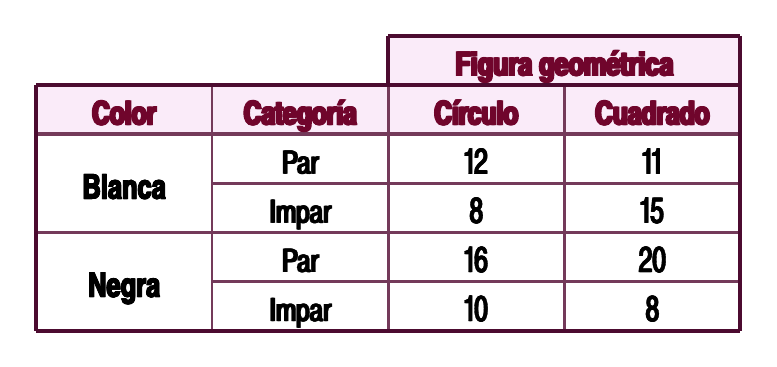
\begin{tikzpicture}[x=0.5pt,y=-0.5pt]
\makeatletter
\definecolor{tfRelleno}{RGB}{250,235,249}
\definecolor{tfVino}{RGB}{112,5,44}
\definecolor{tfLinea}{RGB}{76,11,48}
\definecolor{tfLineaF}{RGB}{116,58,90}
\def\tfFH{\fontsize{11.8pt}{11.8pt}\fontseries{bc}\pgfutil@selectfont}
\def\tfFK{\fontsize{12.2pt}{12.2pt}\fontseries{bc}\pgfutil@selectfont}
\def\tfFR{\fontsize{11.6pt}{11.6pt}\fontseries{c}\pgfutil@selectfont}
\def\tfFN{\fontsize{13.0pt}{13.0pt}\fontseries{c}\pgfutil@selectfont}
\def\tfsxH{0.915}\def\tfsxT{0.938}\def\tfsxK{0.918}\def\tfsxR{0.916}\def\tfsxN{0.825}
\def\tfeH{0.40}\def\tfeK{0.32}\def\tfeR{0.10}\def\tfeN{0.15}
\def\tfsmH{0.65}\def\tfsmK{0.3}\def\tfsmR{0.7}\def\tfsmN{0.5}
\def\tfEon#1{\pgfsys@invoke{2 Tr #1 w}}
\def\tfEoff{\pgfsys@invoke{0 Tr}}
\def\tfU{\setbox0\hbox{1}\hbox to 0.70\wd0{\hss\box0\hss}}
\def\tfN#1#2#3#4#5#6#7{\begin{scope}[shift={(#1,#2)},xscale=#3,transform shape]\node[anchor=base,inner sep=0pt,outer sep=0pt,font=#4,text=#5] at (0,0) {#6#7\tfEoff};\end{scope}}
\def\tfTgen#1#2#3#4#5#6#7#8{\tfN{#1}{#2}{#3}{#4}{#5}{#6}{#7}\ifdim#8pt>0pt\tfN{#1-#8}{#2}{#3}{#4}{#5}{#6}{#7}\tfN{#1+#8}{#2}{#3}{#4}{#5}{#6}{#7}\fi}
\def\tfTT#1#2#3{\tfTgen{#1}{#2}{\tfsxT}{\tfFH}{tfVino}{\tfEon{\tfeH}}{#3}{\tfsmH}}
\def\tfTH#1#2#3{\tfTgen{#1}{#2}{\tfsxH}{\tfFH}{tfVino}{\tfEon{\tfeH}}{#3}{\tfsmH}}
\def\tfTK#1#2#3{\tfTgen{#1}{#2}{\tfsxK}{\tfFK}{black}{\tfEon{\tfeK}}{#3}{\tfsmK}}
\def\tfTR#1#2#3{\tfTgen{#1}{#2}{\tfsxR}{\tfFR}{black}{\tfEon{\tfeR}}{#3}{\tfsmR}}
\def\tfTN#1#2#3{\tfTgen{#1}{#2}{\tfsxN}{\tfFN}{black}{\tfEon{\tfeN}}{#3}{\tfsmN}}
\ifdefined\tfmw\else\newlength{\tfmw}\fi
\def\tfpad{9}\def\tfNecC{0}\def\tfNecT{0}
\def\tfMedC#1#2#3{\settowidth{\tfmw}{#1 #3}\pgfmathsetmacro\tfNecC{max(\tfNecC,2*\tfmw*#2+2*\tfpad)}}
\def\tfMedT#1#2#3{\settowidth{\tfmw}{#1 #3}\pgfmathsetmacro\tfNecT{max(\tfNecT,2*\tfmw*#2+2*\tfpad)}}
\tfMedT{\tfFH}{\tfsxT}{Figura geométrica}
\tfMedC{\tfFH}{\tfsxH}{Color}
\tfMedC{\tfFH}{\tfsxH}{Categoría}
\tfMedC{\tfFH}{\tfsxH}{Círculo}
\tfMedC{\tfFH}{\tfsxH}{Cuadrado}
\tfMedC{\tfFK}{\tfsxK}{Blanca}
\tfMedC{\tfFK}{\tfsxK}{Negra}
\tfMedC{\tfFR}{\tfsxR}{Par}
\tfMedC{\tfFR}{\tfsxR}{Impar}
\tfMedC{\tfFN}{\tfsxN}{\tfU{}2}
\tfMedC{\tfFN}{\tfsxN}{8}
\tfMedC{\tfFN}{\tfsxN}{\tfU{}6}
\tfMedC{\tfFN}{\tfsxN}{\tfU{}0}
\tfMedC{\tfFN}{\tfsxN}{\tfU{}\tfU{}}
\tfMedC{\tfFN}{\tfsxN}{\tfU{}5}
\tfMedC{\tfFN}{\tfsxN}{20}
\pgfmathsetmacro{\tfW}{max(127.25,\tfNecC,\tfNecT/2)}
\pgfmathsetmacro{\tfxa}{10}\pgfmathsetmacro{\tfxb}{\tfxa+\tfW}\pgfmathsetmacro{\tfxc}{\tfxa+2*\tfW}
\pgfmathsetmacro{\tfxd}{\tfxa+3*\tfW}\pgfmathsetmacro{\tfxe}{\tfxa+4*\tfW}
\pgfmathsetmacro{\tfca}{(\tfxa+\tfxb)/2+0.1}\pgfmathsetmacro{\tfcb}{(\tfxb+\tfxc)/2+0.1}
\pgfmathsetmacro{\tfcc}{(\tfxc+\tfxd)/2+0.1}\pgfmathsetmacro{\tfcd}{(\tfxd+\tfxe)/2+0.1}
\pgfmathsetmacro{\tfct}{\tfxd+0.1}
\useasboundingbox (\tfxa-6,10) rectangle (\tfxe+6,235);
\fill[white] (\tfxa-10,6) rectangle (\tfxe+10,239);
\fill[tfRelleno] (\tfxc,16) rectangle (\tfxe,51.5);
\fill[tfRelleno] (\tfxa,51.5) rectangle (\tfxe,87);
\begin{scope}[tfLineaF,line cap=butt]
\draw[line width=1.28pt] (\tfxa,87) -- (\tfxe,87);
\draw[line width=1.28pt] (\tfxb,122.5) -- (\tfxe,122.5);
\draw[line width=1.28pt] (\tfxa,158) -- (\tfxe,158);
\draw[line width=1.28pt] (\tfxb,193.5) -- (\tfxe,193.5);
\draw[line width=1.00pt] (\tfxb,51.5) -- (\tfxb,229);
\draw[line width=1.00pt] (\tfxc,51.5) -- (\tfxc,229);
\draw[line width=1.00pt] (\tfxd,51.5) -- (\tfxd,229);
\end{scope}
\begin{scope}[tfLinea,line cap=projecting]
\draw[line width=1.55pt] (\tfxc,16) -- (\tfxe,16);
\draw[line width=1.55pt] (\tfxa,51.5) -- (\tfxc,51.5);
\draw[line width=1.30pt] (\tfxc,51.5) -- (\tfxe,51.5);
\draw[line width=1.55pt] (\tfxa,229) -- (\tfxe,229);
\draw[line width=1.38pt] (\tfxa,51.5) -- (\tfxa,229);
\draw[line width=1.38pt] (\tfxc,16) -- (\tfxc,51.5);
\draw[line width=1.38pt] (\tfxe,16) -- (\tfxe,229);
\end{scope}
\tfTT{\tfct}{44.45}{Figura geométrica}
\tfTH{\tfca}{79.95}{Color}
\tfTH{\tfcb}{79.95}{Categoría}
\tfTH{\tfcc}{79.95}{Círculo}
\tfTH{\tfcd}{79.95}{Cuadrado}
\tfTK{\tfca}{133.50}{Blanca}
\tfTK{\tfca}{204.50}{Negra}
\tfTR{\tfcb}{115.45}{Par}
\tfTN{\tfcc}{115.45}{\tfU{}2}
\tfTN{\tfcd}{115.45}{\tfU{}\tfU{}}
\tfTR{\tfcb}{150.95}{Impar}
\tfTN{\tfcc}{150.95}{8}
\tfTN{\tfcd}{150.95}{\tfU{}5}
\tfTR{\tfcb}{186.45}{Par}
\tfTN{\tfcc}{186.45}{\tfU{}6}
\tfTN{\tfcd}{186.45}{20}
\tfTR{\tfcb}{221.95}{Impar}
\tfTN{\tfcc}{221.95}{\tfU{}0}
\tfTN{\tfcd}{221.95}{8}
\makeatother
\end{tikzpicture}
\end{document}
